%*******10********20********30********40********50********60********70********80
\chap{Design}
\section{Web application structure}
\vspace{-5mm}
The main page of the application shows you a log in/sign in option, for being able to see your own page and use the functionality. Once you have an account and log in, it shows you a calendar with the days with events in different colors; clicking in the day it shows you all the events to that day, with all the information about that event.\\
Going to the user's page, you will have the calendar again, and you will be able to list all the calendars you own (and add a new one), the events of these timetables, and the events of the timetables you have joined (which you do not own).\\
There will be a \textit{Timetable} bottom for seeing all the timetables in the database. You will be able to search a particular one, go the that timetable page, see all the events and participants, and (in case the timetable would not be yours) join it.\\
In addition, in all pages you will see bottoms to go to \textit{Help}, \textit{About} and \textit{Contact} pages, just in case you need information or making a request.

\newpage

\section{Models design}
\label{Models}
\vspace{-5mm}
\begin{figure}[H]
	\centering
    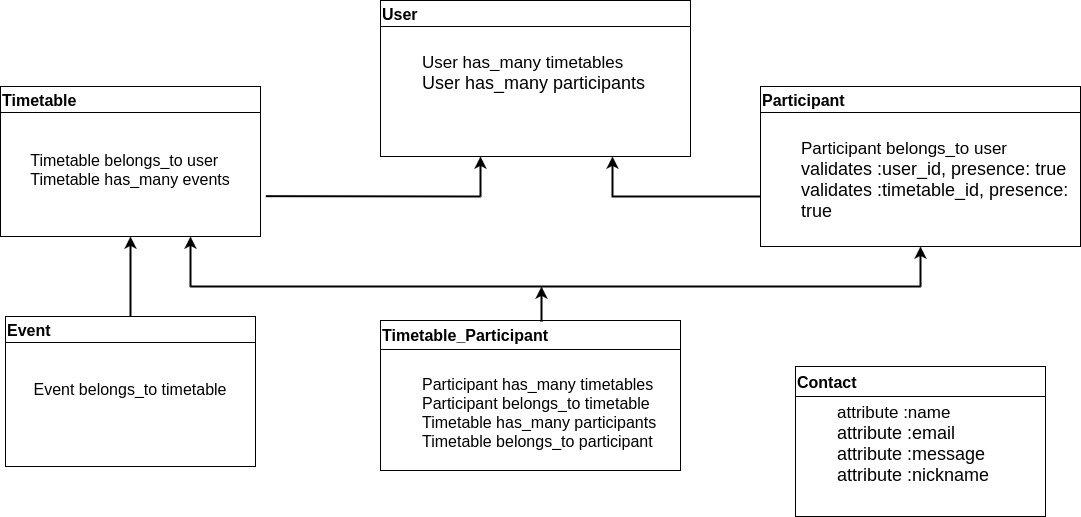
\includegraphics[trim={0 0 0 0},clip,width=1\textwidth]{Files/Models.jpg}
    \caption{Implemented models.\cite{draw:io}}
    \label{fig: Models}
\end{figure}

\subsection{User}
\vspace{-5mm}
The user model is responsible for keeping track of the application's user information. It is directly related to the timetable and participant models, because each user must be able to own several timetables, as well as participating.\\ 
The rest of the model is set up to ensure that the user information is correct. It validates the user e-mail, uses a Bcrypt function to ensure that all users have passwords, and in turn, hashes the password string so that no plaintext passwords are stored in the database. An added feature also allows the user to upload an avatar (profile picture) for their profile. \cite{wiki:RoR}

\subsection{Timetable}
\vspace{-5mm}
The timetable model provide to the users the possibility to set up the general information about a specific schedule. The main utility of the timetable records is to group up the events of the same schedule, allowing users to find and check out the events which they are interested in.
\subsection{Event}
\vspace{-5mm}
The event model allows users to create and record data about a new event of a specific timetable that they own. When ever a owner of a timetable wants to create an event, he has the possibility to do it using this model that provide several active record fields such as name of the events, date of the event, starting time, ending time.. \\
Is important to remember that each single event belongs to a timetable.
\subsection{Participant}
\vspace{-5mm}
The participant model was the last one on implementation, and the most difficult, due to the fact it has relations with two other models:
\begin{itemize} \setlength{\itemsep}{-5pt}
\item Users: a participant is a user. That is, one-to-many relationship.
\item Timetables: many-to-many relationship
\begin{itemize} \setlength{\itemsep}{-5pt}
\item A participant "belongs" to a timetable, but can participate in many timetables.
\item A timetable can have many participants.
\end{itemize}
\end{itemize} 
Obviously, the fields for the foreign keys to user and timetable can not be empty.\\
The many-to-many relation was done separating the "belongs\_to/has\_many" instead using the formula "has\_and\_belongs\_to\_many" because this last one caused us problems in the admin page and when trying to use the foreign keys. These problems were caused  because the use of the foreign key as \textit{user.participant} were not different from \textit{user.participants} (there were not two different relationships).
\subsection{Contact}
\vspace{-5mm}
The contact model is a small and simple one, but it contains the necessary parts for a proper e-mail header. 
Whenever a user submits a new contact form, the model validates the fields of the form, as well as one "invisible" field, 
used for catching spam bots. This "spam catcher" works by refusing to submit forms where the field \textit{nickname} 
contains any characters. Since the field being hidden by some CSS code, we know that a human can't see this field, unless they have access to the code, in which case it's most likely a robot of some kind.
 
